\section{Technical Approach}
To infer information about Java code we use existing inference tools and
combine their output. We have additionally developed a simple framework to aid
in writing our own analyses, should that prove necessary.

To combine the results of disparate analyses we have to convert their results
into a common format at some point in our toolchain.  We will use the JAIF
(Java Annotation Index File) format for that purpose.  Some anaylses generate
results directly in JAIF format, some provide annotated bytecodes which can be
easily extracted into JAIF format, and others provide textual results for which
we will write simple translators into JAIF format.

\begin{figure}
\centering
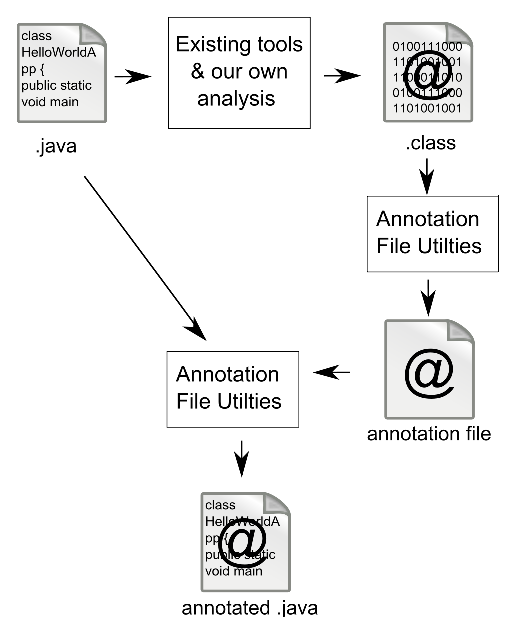
\psfig{file=figures/technicalApproach/technicalApproach.eps, width=3in}
\caption{Toolchain}
\label{fig:toolchain}
\end{figure}

In the following section we describe our simple analysis framework.  In
sections~\ref{sec:Javarifier} through~\ref{sec:Nullability} we describe each of
the existing analyses we will be using in our evaluation and how we will
integrate its results into our toolchain. In section~\ref{sec:jaif2html} we
explain the final step of our process which is to integrate the various
analysis into the Javadoc generation process.

Figure \ref{fig:toolchain} shows the stages in our toolchain.

\subsection{Analysis Framework}
\label{ss:analysisFramework}

To implement our own analysis tools we use the Annotation Processing Tool (APT)
API~\cite{apt} built into the Java standard compiler.  From within an APT plugin
we can access the compiler's abstract syntax tree and augment the generated
bytecode with annotations representing our analysis results. These annotations
are then extracted into external annotation files.


\subsection{From JAIF to HTML documentation}
\label{sec:jaif2html}

Once the results of the various analyses have been collected into a set of
annotation files, we use the annotation file utilities~\cite{AFU} to merge
those annotations back into the original library source. We then use a custom
Javadoc doclet~\cite{doclet} to augment the original Javadoc documentation (if
any) with the information represented by the analysis annotations.

For each analysis, we provide a mapping from the annotation data to either a
textual or iconic representation of the constraints it describes. For example,
a method parameter annotated with \texttt{@Nullable} may result in the text
``(null allowed)'' being appended to the documentation for that parameter. We
will also investigate representing very common annotations such as nullability
in a compact iconic form to avoid overwhelming any existing documentation with
our analysis-derived additions.
